%!TEX encoding = UTF-8 Unicode

%!TEX root = ../compendium1.tex

\Lab{\LabWeekSIX}

\begin{Goals}
%\item Kunna skapa en klass utifrån en textuell beskrivning. % av dess medlemmar.
%\item Kunna skapa en klass utifrån ofärdig kod och dokumentationskommentarer.
%\item Kunna införa privata attribut med lämpliga namn som representerar instansers förändringsbara tillstånd.
\item Kunna förklara skillnader och likheter mellan ett singelobjekt och objekt som är instanser av klasser.
\item Kunna förklara skillnaden mellan förändringsbara och oföränderliga objekt.
\item Kunna definiera och instansiera klasser och case-klasser, samt kunna beskriva när en case-klass är lämpligast och ge några exempel på vad en sådan erbjuder utöver en vanlig klass.
\item Kunna skapa och använda klasser vars instanser innehåller referenser till andra instanser (aggregering).
\item Förstå innebörden av instansreferensen \code{this}.
\item Kunna skapa enkla match-uttryck.
\end{Goals}

\begin{Preparations}
\item \DoExercise{\ExeWeekFIVE}{05}, speciellt uppgift \ref{exe:classes:labprep}.
\item \DoExercise{\ExeWeekSIX}{06}.
\item Läs igenom hela laborationen och planera ditt arbete.
\item Hämta given kod via \href{https://github.com/lunduniversity/introprog/tree/master/workspace/}{kursen github-plats} eller via hemsidan under \href{https://cs.lth.se/pgk/download/}{Download}.

\end{Preparations}

\subsection{Bakgrund}

{\raggedright%
\begin{minipage}{0.42\textwidth}
\begin{figure}[H]
  %\centering
  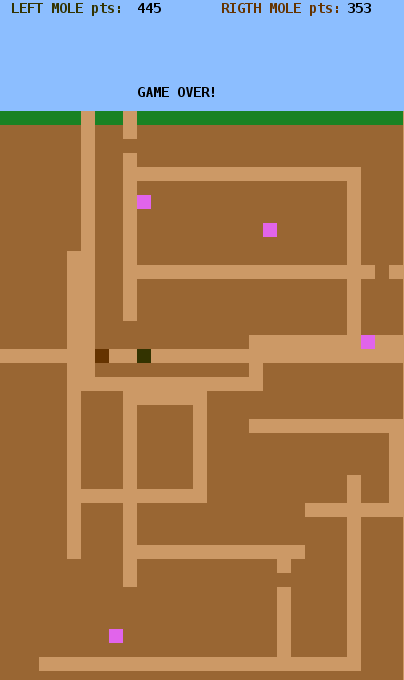
\includegraphics[width=1.0\textwidth]{../img/blockbattle.png}
  \caption{En duell om blockmaskar mellan två lundensiska blockmullvader fångade på bild under intensivt grävanade.}
  \label{lab:blockbattle:fig:game}
\end{figure}
\end{minipage}%
}%
\newlength{\currentparskip}%
\newlength{\currentparindent}%
{
\setlength{\currentparskip}{\parskip}% save the value
\setlength{\currentparindent}{\parindent}% save the value
\hfill%
\begin{minipage}{0.47\textwidth}
\setlength{\parskip}{\currentparskip}% restore the value
\setlength{\parindent}{\currentparindent}% restore the value
\noindent Under denna laboration ska du träna på att deklarera klasser och skapa flera instanser av samma klass. Du tränar även på att bygga ett större program från grunden.

Du ska utveckla ett spel för två spelare som sitter vid samma tangentbord, där den vänstra spelaren styr en blockmullvad med tangenterna A,S,D,W, och den högra spelaren styr en annan blockmullvad med piltangenterna.

I bilden till vänster ser du hur spelet kan se ut. Det finns en ljusbrun och en mörkbrun mullvad. Poängräkningen visas överst i himlen. Det finns fyra rosa blockmaskar (se uppgift \ref{lab:blockmole:task:blockworm} i laboration \code{blockmole}) som mullvadarna tävlar om att försöka fånga. När en blockmask teleporterar sig till en ny slumpmässig position lämnar den jord efter sig. När en mullvad gräver sig upp till gräsytan blir det hål i gräset.
Det ger poäng att gräva tunnlar och att fånga blockmaskar.

Du bestämmer själv hur poängsättningen ska ske och kriteriet för när spelet är slut etc.
\end{minipage}%
}



\subsection{Obligatoriska krav}

Följande funktionella krav ska uppfyllas av ditt program:
\begin{itemize}[nosep, label={$\square$},]
%\item Det ska finnas två blockmullvadar, en för vänster spelare och en för höger spelare, som styrs med ASDW resp. piltangerna.
\item Varje mullvad rör sig i sin aktuella riktning tills användaren ändrar riktning genom att trycka på ''sin'' motsvarande knapp, t.ex. W eller pil-upp.
\item Då en mullvad går i mörkbrun jord ska ljusbruna tunnlar grävas.
\item Då en blockmullvad når fönstrets kant eller himlen ska dess riktning reverseras.
\item Det ska ge poäng att gräva tunnlar.
\item Varje spelares poäng ska visas under spelets gång.
\item Ett spel ska avslutas och \emph{Game over} visas när något valfritt kriterium uppfyllts.
%\item Vid \emph{Game over} ska man kunna välja att avsluta programmet eller spela igen.
\end{itemize}

\noindent Din kod ska utformas enligt dessa design-krav:
\begin{itemize}[nosep, label={$\square$}]
\item Ett \code{Game} skapas i huvudprogrammet med metoden \code{start} som kör igång spelet.
\item Konstanter ska namnges och placeras i lämpligt kompanjonsobjekt.
\item Varje klass med ev. tillhörande kompanjonsobjekt ska finnas i en egen kodfil och tillhöra paketet \code{blockbattle}.
\item Du ska utgå från klasserna som du implementerat i uppgift \ref{exe:classes:labprep} i övning \texttt{\ExeWeekFIVE}.
\item Klassen \code{BlockWindow} omvandlar till interna fönsterkoordinater. Övriga klasser ska använda block-koordinater.
\end{itemize}


\subsection{Valbara krav -- välj minst ett}

Du ska implementera minst ett (gärna flera) av dessa krav:
\begin{itemize}[nosep, label={$\square$}]
\item Det ska finnas lagom många blockmaskar (se labb \code{blockmole} uppg. \ref{lab:blockmole:task:blockworm},  sid. \pageref{lab:blockmole:task:blockworm}).
\item Blockmullvadarna ska även ha ett attribut som representerar hälsan, t.ex. ett numeriskt värde mellan 0 och 100. Hälsan ska försvagas något när man gräver tunnlar. Hälsan ska synas i spelfönstret, t.ex. som en sekvens med röda block i himlen som indikerar andelen av maxhälsan för resp. spelare.
\item Att springa på gräset ska påverka poäng och/eller hälsa.
\item Att fånga blockmask ska påverka poäng och/eller hälsa.
\item Det ska finnas gula blockdiamanter som ger många poäng om man tar dem först.
\item Det ska vid spelstart gå att välja namn på respektive blockmullvad och namnet ska synas i spelet vid poängutskriften.
\item Det ska gå fortare att gå i gångar jämfört med att gräva i jord.
\item Om en blockmullvad fångar en blockmask ska dess grävhastighet öka.
\item Om en blockmullvad krockar med en annan blockmullvad ska något hända, t.ex. att dess riktning reverseras.
\item Visa \emph{highscore} vid \emph{Game Over}.  Highscore sparas med \code{introprog.IO} i en fil som skapas om den inte finns annars läses in vid uppstart om den finns och uppdateras vid behov. Spara hela highscore-listan eller bara högsta poäng hittills.
\end{itemize}

\subsection{Förebredelser inför redovisningen}
\Checkpoint\noindent Innan du redovisar din implementation ska du muntligt kunna redogöra för följande:
\begin{itemize}[nosep, label={$\square$}]
  \item Studera någon annans spel och ge din kamrat minst ett tips om hur kodens läsbarhet kan förbättras. Skriv ner dina tips och beskriv dem vid redovisningen.
  \item Beskriv vilka åtgärder du gjort för att din kod ska vara lätt att läsa och förstå.
  \item Beskriv hur du stegvis utvecklat ditt program från enklare till mer avancerad funktionalitet, samt vilka buggar du upptäckt och fixat.
  \item Beskriv vilket eller vilka valfria krav som din implementation uppfyller.
  \item Beskriv hur du hade behövt ändra i klassen \code{Mole} för att det ska gå att skriva\\\code{new Mole().move().move().reverseDir().move()}
\end{itemize}

\subsection{Tips och förslag}

\begin{enumerate}[leftmargin=*]
  \item \textbf{Många små steg.} Kör kompilering under ändringsbevakning med \code{--watch} i ett eget terminalfönster, så att du vid varje ändring kan rätta ev. kompileringsfel. Kör och testa ditt program ett annat terminalfönster.

  \item \textbf{Inför bra namn}. Din kod blir lättare att läsa och ändra i om du hittar på bra namn på medlemmar och lägger dem på lämpligt ställe. T.ex. kan du samla globala spel-konstanter i kompanjonsobjektet till klassen \code{Game}. Du kan bygga vidare på nedan kod och lägga till medlemmar allteftersom du upptäcker att de behövs. Nedan finns exempelvis en funktion som ger bakgrundsfärgen för en viss y-koordinat, vilken är användbar när du ska återställa bakgrunden efter att en mullvad har flyttat sig.
\scalainputlisting[basicstyle=\ttfamily\fontsize{10}{12}\selectfont]{../workspace/w06_blockbattle/Game.scala}
% \begin{CodeSmall}
% object Game {
%   val windowSize = (30, 50)
%   val windowTitle = "EPIC BLOCK BATTLE"
%   val blockSize = 14
%   val skyRange    = 0 to 7
%   val grassRange  = 8 to 8
%   object Color { ??? }
%   def backgroundColorAtDepth(y: Int): java.awt.Color = ???
% }
%
% class Game(
%   val leftPlayerName: String  = "LEFT",
%   val rightPlayerName: String = "RIGHT"
% ) {
%  import Game.* // direkt tillgång till namn på medlemmar i kompanjon
%
%  val window    = new BlockWindow(windowSize, windowTitle, blockSize)
%  val leftMole  = ???
%  val rightMole = ???
%
%  def drawWorld(): Unit = ???
%
%  def eraseBlocks(x1: Int, y1: Int, x2: Int, y2: Int): Unit = ???
%
%  def update(mole: Mole): Unit = ???  // update, draw new, erase old
%
%  def gameLoop(): Unit = ???
%
%  def start(): Unit = {
%    println("Start digging!")
%    println(s"$leftPlayerName ${leftMole.keyControl}")
%    println(s"$rightPlayerName ${rightMole.keyControl}")
%    drawWorld()
%    gameLoop()
%  }
% }
% \end{CodeSmall}

 \item \textbf{Dela upp din kod i funktioner.} Din kod blir lättare att läsa och ändra i om du delar upp den i många små funktioner med bra namn. I \code{Game}-klassen ovan finns exempel på några användbara funktioner. Allteftersom du utvidgar ditt program kan du lägga till fler funktioner som t.ex. heter \code{showPoints}, \code{gameOver}, etc.

\item \textbf{Tänk igenom den övergripande strukturen.} Programmet du ska skriva i denna laboration är större än det du gjort tidigare. Det är därför viktigt att tänka igenom strukturen på ditt program, vilka klasser som har hand om vad och hur de samarbetar. Diskutera gärna med handledare om du är osäker på hur de koddelar du utvecklat i föregående veckas övning \ref{exe:classes:labprep}, klasserna \code{Pos}, \code{KeyControl}, \code{Mole} och \code{BlockWindow}, är tänkta att samverka. Var noga med att testa så de olika klasserna och deras metoder fungerar var för sig.     

\item \textbf{Utformning av \texttt{gameLoop()}}. I ett spel behövs en s.k. spel-loop \Eng{game loop} som upprepar den kod som ska köras vid varje ny skärmbild, ofta kallad \emph{frame}. I varje runda i spel-loopen sker uppdatering av data och ritning i spelfönstret, samt en lämplig fördröjning. En skiss på en typisk spel-loop visas nedan:
\begin{CodeSmall}
  var quit = false
  val delayMillis = 80

  def gameLoop(): Unit = 
    while !quit do
      val t0 = System.currentTimeMillis
      handleEvents()    // ändrar riktning vid tangenttryck etc.
      update(leftMole)  // flyttar, ritar, suddar, etc.
      update(rightMole)

      val elapsedMillis = (System.currentTimeMillis - t0).toInt
      Thread.sleep((delayMillis - elapsedMillis) max 0)
    end while
  end gameLoop
\end{CodeSmall}

\item \textbf{Hantering av händelser.} Ett \code{BlockWindow}, som du implementerade i uppgift \ref{exe:classes:labprep} i övning \texttt{\ExeWeekFIVE}, kan via anrop av \code{nextEvent} ge   \code{KeyPressed(key)} vid knapptryck och \code{WindowClosed} vid fönsterstängning. Om ingen händelse finns att behandla returneras \code{Undefined}. Använd en loop som betar av alla händelser tills \code{Undefined} påträffas, enligt nedan:

\begin{CodeSmall}
  def handleEvents(): Unit = 
    var e = window.nextEvent()
    while e != BlockWindow.Event.Undefined do
      e match 
        case BlockWindow.Event.KeyPressed(key) =>
          ???  // ändra riktning på resp. mullvad

        case BlockWindow.Event.WindowClosed =>
          ???  // avsluta spel-loopen
      
      e = window.nextEvent()
    end while
  end handleEvent
\end{CodeSmall}

\item \textbf{Flimmerfri grafik.} För att minska mängden flimmer \Eng{flicker} är det bäst att i varje iteration i spel-loopen (1) bara rita om det som ändrats för att minimera tiden som spenderas på att rita, och (2) vid ändringar rita nya delar före att gamla delar raderas. För att slippa mullvadsflimmer kan du ''\emph{rita först -- sudda sen}'' enligt nedan.\footnote{Inom spelutveckling använder man oftast istället så kallad \emph{double buffering} (eller till och med \emph{triple buffering}) för att få helt flimmerfri grafik. Det ligger dock bortom kursen och stöds inte av \code{PixelWindow}.}

% \begin{CodeSmall}
% val oldMolePos = mole.pos                  // save
% mole.move()                                // update
% window.setBlock(mole.pos, mole.color)      // draw new
% window.setBlock(oldMolePos, Color.tunnel)  // erase old
% \end{CodeSmall}

\begin{CodeSmall}
window.setBlock(mole.nextPos, mole.color) // draw new
window.setBlock(mole.pos, Color.tunnel)   // erase old
mole.move()                               // update
\end{CodeSmall}

\end{enumerate}
